\chapter{Menyiapkan PostgreSQL dan Phoenix Framework}

Pada bab ini, akan dijelaskan proses instalasi dan konfigurasi PostgreSQL, menyiapkan Phoenix Framework, serta membuat aplikasi web sederhana. Ini mencakup pendefinisian rute, pembuatan controller, dan rendering template HTML.

\section{Pengenalan Phoenix Framework}
Phoenix Framework adalah framework pengembangan web modern yang lengkap, dibangun di atas bahasa pemrograman Elixir. Phoenix dirancang untuk menangani kebutuhan aplikasi berskala besar dan real-time dengan mudah, berkat kecepatan dan skalabilitasnya. Phoenix memanfaatkan model konkruensi Elixir yang berbasis pada mesin virtual Erlang (BEAM), menjadikannya pilihan yang sangat baik untuk aplikasi yang membutuhkan ketersediaan tinggi dan fungsionalitas real-time, seperti aplikasi percakapan, platform permainan daring, dan dasbor interaktif.

Pada intinya, Phoenix mengikuti pola arsitektur Model-View-Controller (MVC), yang memberikan pemisahan yang jelas antara logika aplikasi, data, dan presentasi. Phoenix juga menekankan pengembangan aplikasi konkuren dan terdistribusi dengan memungkinkan sistem tahan kesalahan yang mampu menangani jutaan koneksi secara bersamaan.

Phoenix menawarkan:
\begin{itemize}
	\item Siklus permintaan/tanggapan yang cepat.
	\item Dukungan untuk komunikasi real-time melalui WebSockets.
	\item Dukungan bawaan untuk operasi basis data melalui Ecto, pembungkus basis data dan generator query-nya.
	\item Rendering HTML melalui template dan kode Elixir yang tertanam (HEEx templates).
\end{itemize}

Aplikasi Phoenix dikompilasi ke kode asli, memungkinkan performa yang luar biasa bahkan di bawah beban berat, menjadikannya pilihan yang baik untuk aplikasi web dengan kinerja tinggi. Fokusnya pada produktivitas pengembang dan arsitektur kode yang dapat dipelihara membuat Phoenix cocok untuk proyek dengan berbagai ukuran.

\section{Memahami Pola MVC pada Phoenix}

\begin{figure}[h]
	\begin{center}
		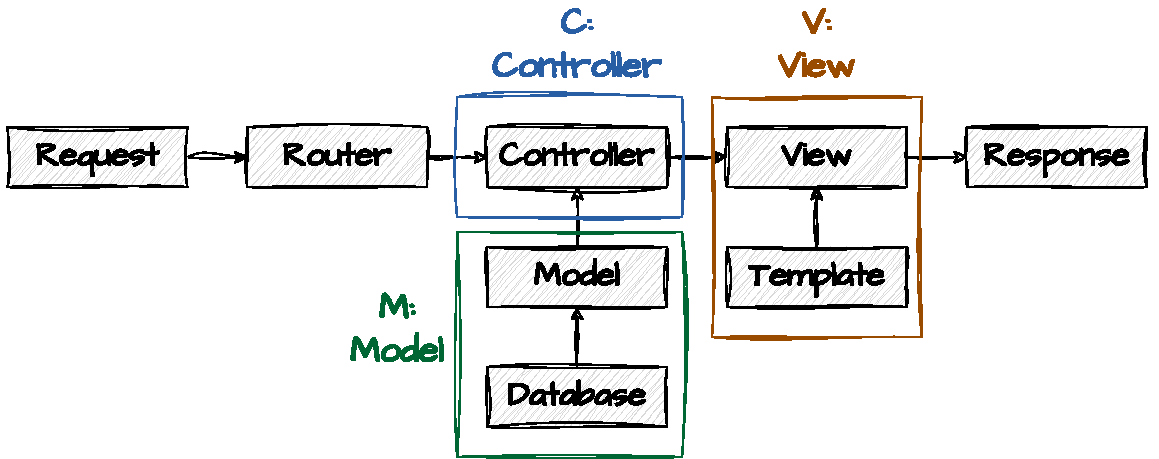
\includegraphics[width=1\textwidth]{../assets/phoenix-mvc.pdf}
	\end{center}
	\caption{MVC pada Phoenix Framework.}
\end{figure}

Phoenix Framework mengimplementasikan pola Model-View-Controller (MVC), yang memisahkan lapisan-lapisan aplikasi untuk mempromosikan kemampuan pemeliharaan, penggunaan ulang, dan kejelasan struktur aplikasi. Berikut adalah bagaimana Phoenix mengimplementasikan MVC dan menangani permintaan web:

\subsection{Penanganan Permintaan pada Phoenix}
Saat seorang pengguna melakukan permintaan ke aplikasi Phoenix, framework ini mengikuti jalur yang terdefinisi dengan baik untuk memproses permintaan tersebut. Proses ini biasanya melalui tahap-tahap berikut:
\begin{enumerate}
	\item \texttt{Router} menerima permintaan dan menentukan controller mana yang harus menanganinya.
	\item \texttt{Controller} menangani logika bisnis dari permintaan tersebut. Controller mungkin berinteraksi dengan \texttt{Model} dan mengambil data dari \texttt{Database}.
	\item \texttt{View} mengambil data dari \texttt{Controller} dan mempersiapkannya untuk ditampilkan dengan merender \texttt{Template} yang sesuai.
	\item \texttt{Response} kemudian dikirim kembali ke klien, biasanya dalam bentuk halaman HTML atau tanggapan JSON.
\end{enumerate}


\subsection{Request}

A request in Phoenix begins when a client, such as a web browser,  
sends an HTTP request to the server. The router identifies the correct  
controller and action to handle it. The request typically contains  
information such as the path, method, headers, and parameters.  

The controller receives this data through the \texttt{conn} struct,  
processes it, and passes the result to the view for rendering the  
final response.

\begin{lstlisting}[language=bash]
GET /about HTTP/1.1
Host: localhost:4000
User-Agent: Mozilla/5.0
Accept: text/html
\end{lstlisting}

This request is routed to \texttt{PageController.about/2},  
which prepares data for the view.


\subsection{Router}
Router bertanggung jawab untuk memetakan permintaan HTTP ke controller dan aksi yang sesuai. Pada Phoenix, rute didefinisikan dalam file \texttt{router.ex}. Router memeriksa jalur dan metode (GET, POST, dll.) dari permintaan yang masuk dan memutuskan controller mana yang harus menangani permintaan tersebut serta aksi (fungsi) mana di dalam controller yang harus dijalankan. Sebagai contoh:

\begin{lstlisting}[language=Elixir]
	scope "/", HelloWeb do
	pipe_through :browser
	
	get "/", PageController, :home
	get "/about", PageController, :about
	get "/queue/new", QueueController, :new
	end
\end{lstlisting}

Kode routing ini memetakan permintaan HTTP GET ke URL seperti \texttt{/about} dan \texttt{/queue/new} ke aksi controller yang sesuai, yang akan menangani logika bisnis untuk jalur tersebut.

\subsection{Controller}
Controller dalam Phoenix berfungsi sebagai penghubung antara model (data) dan view (presentasi). Controller memproses permintaan yang masuk dengan memanggil fungsi yang sesuai, sering kali berinteraksi dengan basis data dan mengembalikan hasilnya ke view.

Sebagai contoh, \texttt{PageController} berikut mendefinisikan dua aksi: \texttt{home} dan \texttt{about}, yang menangani permintaan untuk menampilkan halaman utama dan halaman about, masing-masing.

\begin{lstlisting}[language=Elixir]
	defmodule HelloWeb.PageController do
	use HelloWeb, :controller
	
	def about(conn, _params) do
	render(conn, :about, layout: false)
	end
	
	def home(conn, _params) do
	render(conn, :home, layout: false)
	end
	end
\end{lstlisting}

Dalam hal ini, controller menggunakan fungsi \texttt{render/3} untuk mengembalikan template HTML yang sesuai untuk tanggapan. Argumen \texttt{conn} mewakili koneksi, yang berisi data permintaan dan rincian tanggapan.

\subsection{Model dan Interaksi Basis Data}
Model dalam Phoenix bertanggung jawab untuk merepresentasikan dan mengelola data aplikasi, yang biasanya disimpan dalam basis data. Phoenix menggunakan Ecto, sebuah pembungkus basis data yang kuat dan generator query, untuk berinteraksi dengan basis data. Model biasanya didefinisikan sebagai skema Ecto, yang memetakan struct Elixir ke tabel basis data.

Sebagai contoh, skema dapat terlihat seperti ini:
\begin{lstlisting}[language=Elixir]
	defmodule Hello.Accounts.User do
	use Ecto.Schema
	
	schema "users" do
	field :name, :string
	field :email, :string
	field :age, :integer
	
	timestamps()
	end
	end
\end{lstlisting}

Di sini, skema mendefinisikan model \texttt{User}, yang dipetakan ke tabel \texttt{users} dalam basis data, dengan field \texttt{name}, \texttt{email}, dan \texttt{age}. Melalui Ecto, Phoenix dapat melakukan operasi CRUD (Create, Read, Update, Delete) pada data menggunakan model ini.

\subsection{View dan Template}
View dalam Phoenix bertanggung jawab untuk merender tanggapan dalam format yang sesuai untuk klien, baik itu HTML, JSON, atau format lainnya. View mengambil data yang dikirimkan dari controller dan menerapkan template untuk menghasilkan tanggapan akhir.

View Phoenix biasanya menggunakan HEEx (HTML Embedded Elixir), sebuah mesin templating yang memungkinkan penyisipan kode Elixir di dalam HTML. Berikut adalah contoh template untuk halaman \texttt{about}:

\begin{lstlisting}[language=html]
	<h1><b>Hello World!</b></h1>
\end{lstlisting}

View dirancang untuk menjadi "dumb" dalam artian tidak mengandung logika bisnis. Mereka hanya menyajikan data dalam format yang ditentukan oleh template.

\subsection{Response}
Setelah view memproses data dan menerapkan template, tanggapan akhir dihasilkan dan dikirim kembali ke klien. Tanggapan ini dapat berupa halaman HTML, objek JSON, atau jenis konten lain tergantung pada permintaan dan aksi yang diambil.

Sebagai contoh, jika pengguna meminta halaman \texttt{/about}, server akan mengembalikan tanggapan HTML yang berisi konten template \texttt{about.html.heex}. Klien (biasanya peramban web) kemudian akan merender tanggapan ini sebagai halaman HTML.

\subsection{Menggabungkan Semua Komponen}
Untuk meringkas alur MVC:
\begin{enumerate}
	\item \texttt{Router} menerima permintaan HTTP dan meneruskannya ke \texttt{Controller} yang sesuai.
	\item \texttt{Controller} menangani logika bisnis, mungkin dengan mengambil atau memperbarui data menggunakan \texttt{Model}.
	\item \texttt{View} mengambil data yang disediakan oleh \texttt{Controller} dan menggunakan \texttt{Template} untuk merender tanggapan.
	\item \texttt{Response} dikirim kembali ke klien, melengkapi siklus permintaan/tanggapan.
\end{enumerate}

Dengan memisahkan aplikasi ke dalam komponen-komponen ini, Phoenix memastikan bahwa setiap bagian dari aplikasi terfokus pada satu tanggung jawab, sehingga lebih mudah untuk dipelihara dan ditingkatkan seiring waktu.


\section{Menginstal PostgreSQL}
PostgreSQL adalah sistem basis data objek-relasional open-source yang kuat. PostgreSQL akan digunakan sebagai basis data untuk aplikasi web Phoenix yang akan kita buat. Untuk menginstal PostgreSQL, ikuti langkah-langkah berikut:

\begin{enumerate}
	\item Perbarui daftar paket:
	\begin{lstlisting}[language=bash]
		sudo apt update
	\end{lstlisting}
	
	\item Instal PostgreSQL dan bersihkan konfigurasi lama:
	\begin{lstlisting}[language=bash]
		sudo apt install postgresql -y --purge
	\end{lstlisting}
	
	\item Aktifkan dan mulai layanan PostgreSQL:
	\begin{lstlisting}[language=bash]
		sudo systemctl enable postgresql
		sudo systemctl start postgresql
		sudo systemctl status postgresql
	\end{lstlisting}
	
	\item Instal pgAdmin4 (opsional, untuk manajemen grafis PostgreSQL):
	\begin{lstlisting}[language=bash]
		sudo apt install pgadmin4-desktop -y --purge
	\end{lstlisting}
	
	\item Masuk sebagai pengguna PostgreSQL:
	\begin{lstlisting}[language=bash]
		sudo -i -u postgres
	\end{lstlisting}
	
	\item Atur kata sandi untuk pengguna \texttt{postgres} (untuk pengembangan, atur ke \texttt{1234}):
	\begin{lstlisting}[language=bash]
		psql> \password postgres
	\end{lstlisting}
\end{enumerate}

\section{Menginstal Phoenix Framework}
Phoenix Framework, yang dibangun di atas Elixir, memungkinkan pengembangan aplikasi web yang sangat skalabel. Ikuti langkah-langkah ini untuk menginstal Phoenix dan membuat proyek baru:

\begin{enumerate}
	\item Instal \texttt{inotify-tools} agar Phoenix dapat mendeteksi perubahan file:
	\begin{lstlisting}[language=bash]
		sudo apt install inotify-tools
	\end{lstlisting}
	
	\item Periksa versi Elixir:
	\begin{lstlisting}[language=bash]
		elixir -v
	\end{lstlisting}
	
	\item Instal Hex, manajer paket untuk Elixir:
	\begin{lstlisting}[language=bash]
		mix local.hex
	\end{lstlisting}
	
	\item Instal generator proyek Phoenix:
	\begin{lstlisting}[language=bash]
		mix archive.install hex phx_new
	\end{lstlisting}
	
	\item Buat proyek Phoenix baru bernama \texttt{hello}:
	\begin{lstlisting}[language=bash]
		mix phx.new hello
	\end{lstlisting}
	
	\item Masuk ke direktori proyek dan buka di Visual Studio Code:
	\begin{lstlisting}[language=bash]
		cd hello
		code .
	\end{lstlisting}
	
	\item Edit file konfigurasi basis data \texttt{config/dev.exs} dan \texttt{config/test.exs}, atur kata sandi pengguna \texttt{postgres} ke \texttt{1234}.
	
	\item Dapatkan dependensi proyek dan buat basis data:
	\begin{lstlisting}[language=bash]
		mix deps.get
		mix ecto.create
	\end{lstlisting}
	
	\item Mulai server Phoenix:
	\begin{lstlisting}[language=bash]
		mix phx.server
		iex -S mix phx.server
	\end{lstlisting}
\end{enumerate}

\section{Routing pada Phoenix}
Routing pada Phoenix menentukan bagaimana permintaan yang masuk dipetakan ke controller dan aksi tertentu. Untuk mengkonfigurasi rute aplikasi, ikuti langkah-langkah berikut:

\begin{enumerate}
	\item Buka file \texttt{lib/hello\_web/router.ex} dan definisikan rute berikut:
	\begin{lstlisting}[language=Elixir]
		scope "/", HelloWeb do
		pipe_through :browser
		
		get "/", PageController, :home
		get "/about", PageController, :about
		get "/queue/new", QueueController, :new
		end
	\end{lstlisting}
	
	\item Penjelasan:
	\begin{itemize}
		\item \texttt{pipe\_through :browser}: Ini menerapkan stack browser default pada rute ini, termasuk sesi, cookie, dan penanganan permintaan.
		\item \texttt{get "/"}: Ini memetakan URL root ke aksi \texttt{home} di \texttt{PageController}.
		\item Begitu juga, \texttt{get "/about"} dan \texttt{get "/queue/new"} mendefinisikan rute untuk halaman about dan halaman antrian baru.
	\end{itemize}
\end{enumerate}

\section{Membuat Page dan Queue Controllers}
Controller pada Phoenix menangani logika dan rendering untuk halaman web yang berbeda. Mari kita definisikan dua controller: satu untuk halaman umum dan satu lagi untuk menangani aksi antrian.

\begin{enumerate}
	\item Definisikan \texttt{PageController} untuk menangani halaman utama dan halaman about:
	\begin{lstlisting}[language=Elixir]
		defmodule HelloWeb.PageController do
		use HelloWeb, :controller
		
		def about(conn, _params) do
		render(conn, :about, layout: false)
		end
		
		def home(conn, _params) do
		render(conn, :home, layout: false)
		end
		end
	\end{lstlisting}
	
	\item Penjelasan:
	\begin{itemize}
		\item \texttt{use HelloWeb, :controller}: Ini mengimpor fungsionalitas yang diperlukan untuk mendefinisikan controller Phoenix.
		\item \texttt{about/2}: Fungsi ini merender template \texttt{about.html.heex} tanpa layout.
		\item \texttt{home/2}: Fungsi ini merender template \texttt{home.html.heex}.
	\end{itemize}
	
	\item Definisikan \texttt{QueueController} untuk menangani halaman antrian baru:
	\begin{lstlisting}[language=Elixir]
		defmodule HelloWeb.QueueController do
		use HelloWeb, :controller
		
		def new(conn, _params) do
		render(conn, :new, layout: false)
		end
		end
	\end{lstlisting}
	
	\item Penjelasan:
	\begin{itemize}
		\item \texttt{new/2}: Fungsi ini merender template \texttt{new.html.heex} untuk halaman antrian baru.
	\end{itemize}
\end{enumerate}

\section{Merender Halaman HTML}
Template HTML mendefinisikan struktur halaman web yang dirender oleh controller. Mari kita buat dua template, satu untuk halaman about dan satu lagi untuk halaman antrian baru.

\begin{enumerate}
	\item Buat template \texttt{about.html.heex}:
	\begin{lstlisting}[language=html]
		<h1><b>Hello World!</b></h1>
	\end{lstlisting}
	
	\item Penjelasan:
	\begin{itemize}
		\item Template HTML ini menampilkan pesan "Hello World" sederhana untuk halaman about.
	\end{itemize}
	
	\item Buat template \texttt{new.html.heex} untuk halaman antrian baru:
	\begin{lstlisting}[language=html]
		<h1><b>Ini adalah halaman untuk antrian baru</b></h1>
	\end{lstlisting}
	
	\item Penjelasan:
	\begin{itemize}
		\item Template ini menampilkan judul sederhana untuk halaman antrian baru.
	\end{itemize}
\end{enumerate}

\section{Menyematkan Template}
Phoenix memungkinkan Anda untuk menyematkan template HTML di dalam modul, yang menyederhanakan proses pengelolaan beberapa template untuk sebuah controller.

\begin{enumerate}
	\item Definisikan modul \texttt{QueueHTML} untuk menyematkan template untuk \texttt{QueueController}:
	\begin{lstlisting}[language=Elixir]
		defmodule HelloWeb.QueueHTML do
		@moduledoc """
		Modul ini berisi halaman-halaman yang dirender oleh PageController.
		
		Lihat direktori `queue_html` untuk semua template yang tersedia.
		"""
		use HelloWeb, :html
		
		embed_templates "queue_html/*"
		end
	\end{lstlisting}
	
	\item Penjelasan:
	\begin{itemize}
		\item \texttt{embed\_templates}: Makro ini secara otomatis mengimpor semua template yang ada di direktori \texttt{queue\_html}, menyederhanakan proses rendering halaman.
	\end{itemize}
\end{enumerate}

\section{Kesimpulan}
Dengan mengikuti langkah-langkah ini, Anda telah berhasil menginstal PostgreSQL, menyiapkan aplikasi Phoenix, mendefinisikan rute, membuat controller, dan merender halaman HTML. Pengaturan ini memberikan fondasi untuk pengembangan lebih lanjut dari aplikasi web.
